\chapter{Microsoft Azure}
Platforma została oddana do użytku w 2008 roku jako Windows Azure.\ Usługa ta została zbudowana na modułach Windows NT.\ Platforma została udostępniona komercyjnie po 2010 roku, kiedy to dodano możliwość korzystania z szerszej ilości usług i języków programowania.\ Do usług należało między innymi udostępnienie baz danych Microsoft SQL Server opartych o .NET Framework 4, obsługę aplikacji pisanych w wielu języku (takich jak \textit{C\#}, \textit{Java}, \textit{PHP}), sieć dostarczania zawartości \trans{ang. Content Delivery Network, CDN}.
\\ \\
Następnym krokiem było przemianowanie platformy na Microsoft Azure oraz pójście w kierunku infrastruktury definiowanej jako serwis \trans{ang. Infrastructure-as-a-Service, IaaS}, oraz powolne adoptowanie usług open-source.
\\ \\
W kolejnej generacji Microsoft zaadoptował rozwiązania Big Data do swojej platformy, umożliwiając korzystanie z języka \textit{R}, połączenie do Power BI, a także umożliwienie połączenia do rozwiązań end-to-end.
\\ \\
W czwartej generacji platformy, Microsoft skupił się na rozwiązaniach uczenia maszynowego oraz integracji z bazami danych, dzięki czemu powstało Azure Machine Learning Studio oraz Azure Machine Learning Operations (MLOps).
\\ \\
Obecnie platforma została wzbogacona o Kubernetesa, dzięki czemu konteneryzacja ułatwiła pracę z klastrami wirtualnymi.\ Wirtualne klastry pozwalają na wydajniejszy i wygodniejszy sposób zarządzania aplikacjami i usługami.\ Dodatkowo zostało udostępnione wiele kombinacji usług takich jak: aplikacja jako usługa \trans{ang. Software-as-a-Service} (SaaS), Interfejs jako usługa \trans{ang. Infrastucture-as-a-Service} (IaaS), Platforma jako usługa \trans{ang. Platfrom-as-a-Service} (PaaS).\ Microsoft uzyskał w ten sposób platformę przyjazną użytkownikowi, która umożliwia użytkownikom korzystanie z ponad 200 dostępnych usług.\ Dodatkowo płatność za platformę jest rozliczana tylko za zużytą przestrzeń oraz wykorzystaną moc obliczeniową~\cite{Roosevelt2022, MicrosoftAzurec, Datashift}.

\vfill
\pagebreak

\begin{figure}[H]
    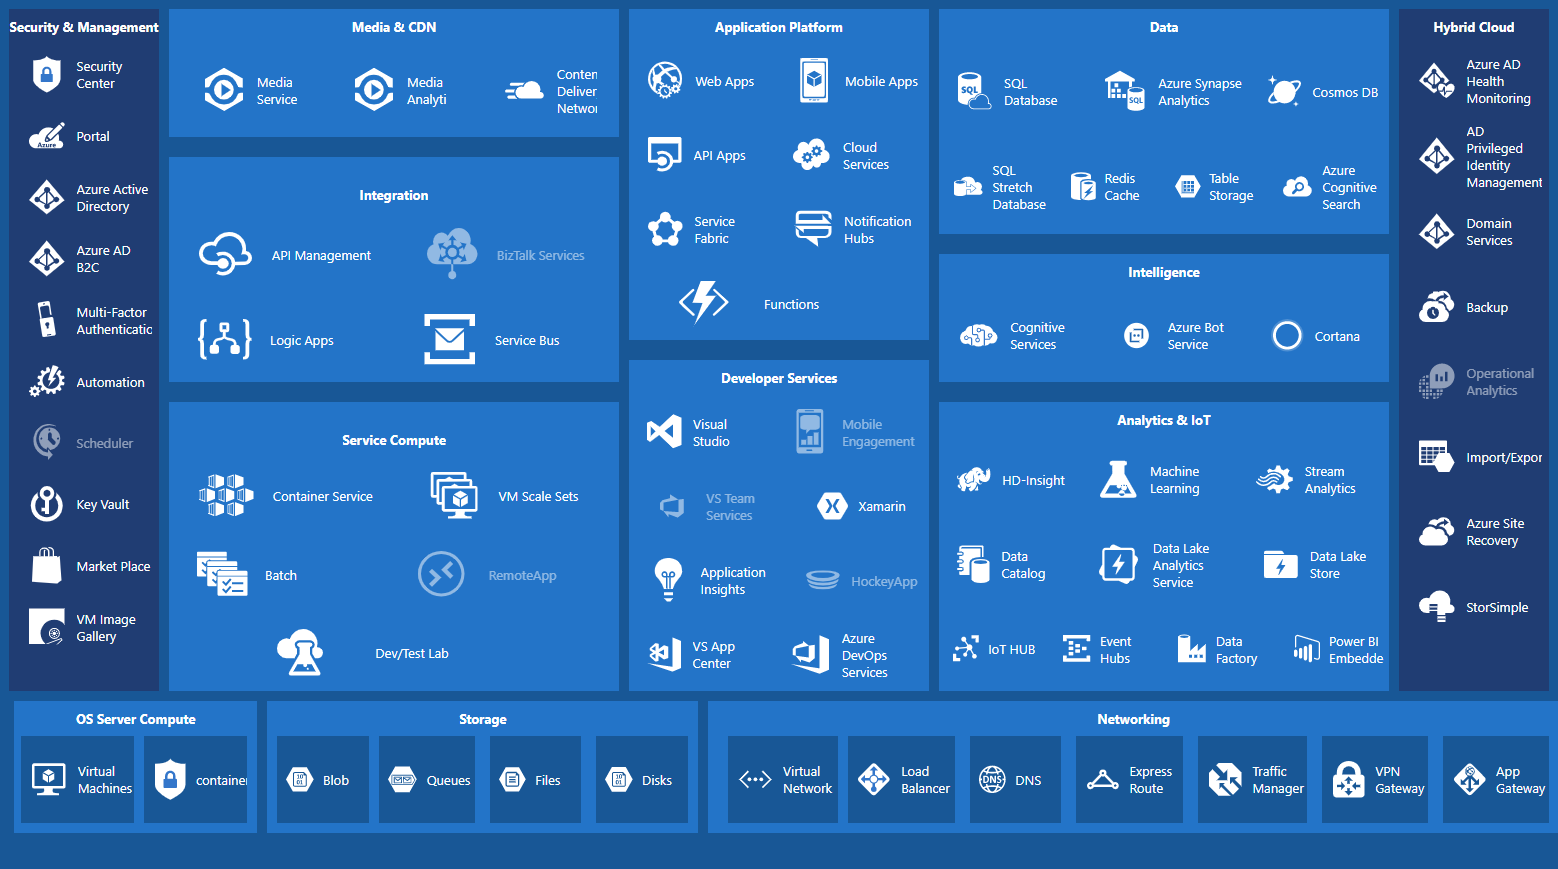
\includegraphics[width=\textwidth]{images/ms_azure}
    \captionsource{Schemat podziału usług MS Azure}{\cite{Datashifta}}
    \label{fig:ms-azure}
\end{figure}

\refsource{Schemat}{fig:ms-azure} pokazuje jak obecnie podzielone są usługi oraz co jest udostępnione komercyjnie w ramach platformy Azure.\ Według schematu platforma podzielona jest na trzynaście obszarów, do których zaliczono między innymi bezpieczeństwo, zarządzanie danymi, usługi deweloperskie, analiza danych, platformy aplikacji.

\section{Infrastruktura}
Infrastruktura globalna Azure składa się z dwóch części: fizycznej infrastruktury oraz globalnej łączności.\ Infrastruktura fizyczna składa się z ponad 200 centrów danych na całym świecie, połączonych w jedną globalną sieć.\ Takie rozwiązanie umożliwia wysoką skalowalność i dostępność poszczególnych rozwiązań.\ Cały ruch sieciowy jest utrzymywany wewnątrz prywatnej sieci Microsoft.\ Pozwala to na zachowanie informacje o adresach IP wewnątrz sieci, a co za tym idzie, informacje te nie trafiają do opinii publicznej~\cite{MicrosoftAzureb}.\\ \\

Na swojej stronie internetowej Microsoft udostępnia wirtualną mapę, umożliwiającą zobaczenie aktualnej sieci Microsoftu oraz jej rozmieszczenie na globie ziemskim.\ Interaktywna mapa pozwala uzyskiwać informację o poszczególnych krajach oraz centrach danych znajdujących się na terytoriach tych krajów.\ Mapę oraz informację pokazano na \refsource{zdjęciach}{fig:azure-ic}.

\vfill
\pagebreak

\begin{figure}[H]
    \begin{subfigure}[m]{0.7\textwidth}
    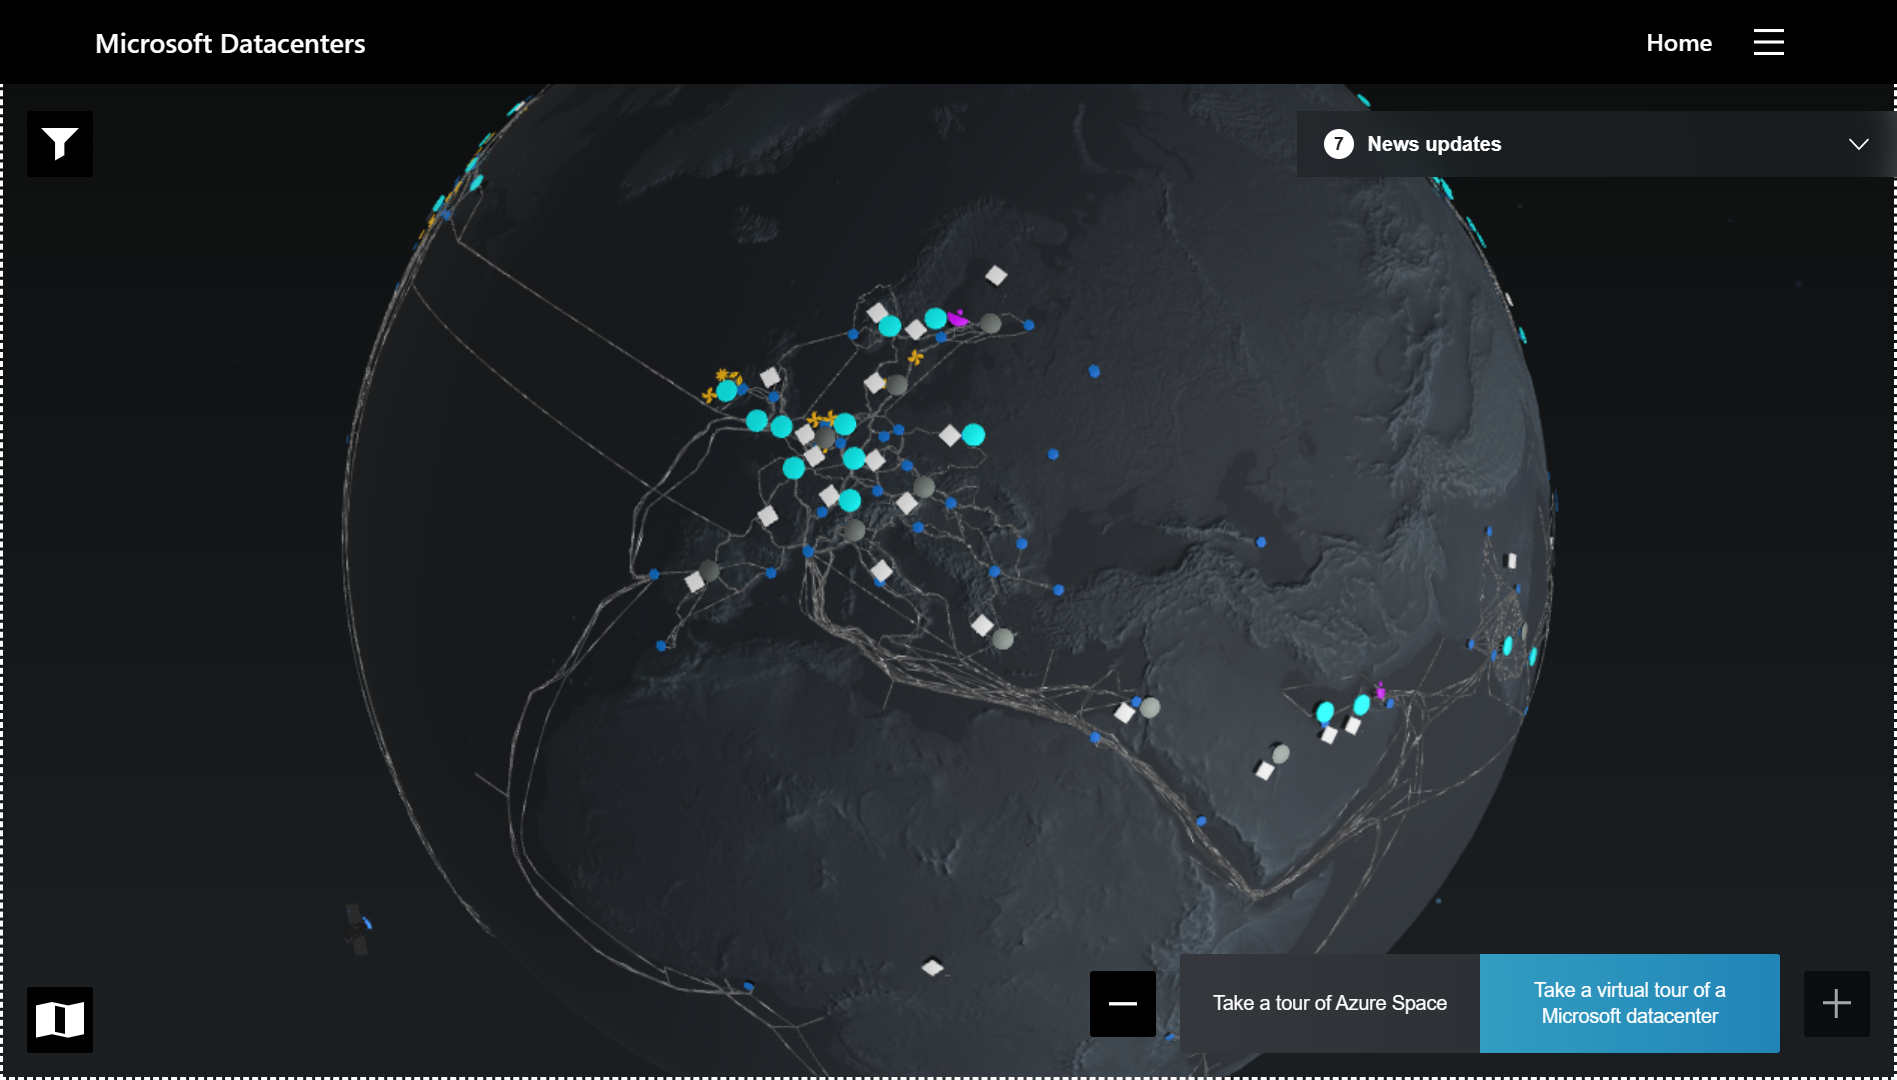
\includegraphics[width=\textwidth]{images/azure-ic}
    \captionsource{Globalna mapa infrastruktury sieciowe}{\cite{MicrosoftAzured}}
    \end{subfigure}
    \hfill
    \begin{subfigure}[m]{0.25\textwidth}
        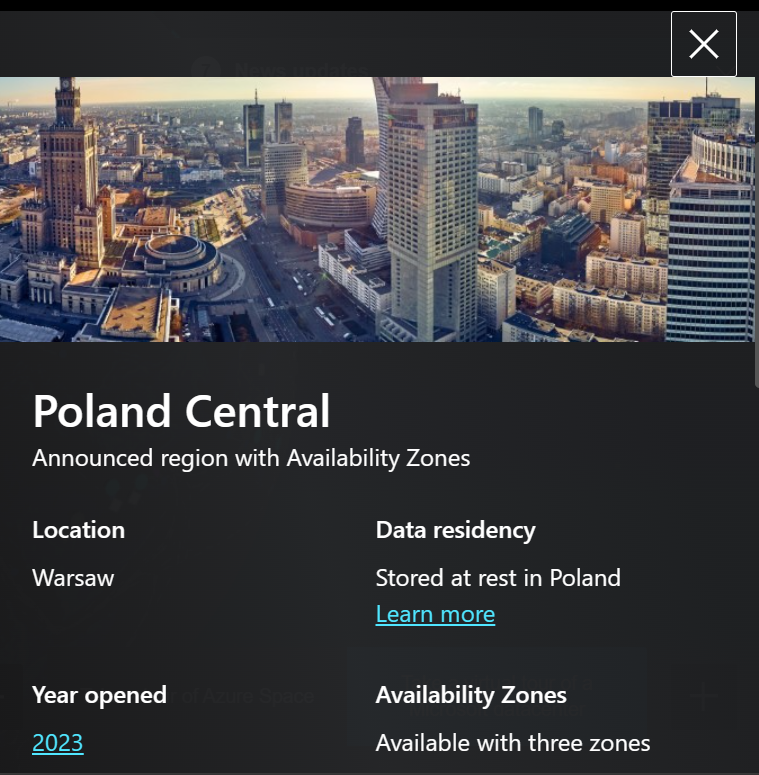
\includegraphics[width=\textwidth]{images/azure-pl}
        \captionsource{Informacje o centrum danych}{\cite{MicrosoftAzuree}}
    \end{subfigure}
    \captionsource{Zdjęcia z mapy insfrastruktury Microsoft Azure}{\cite{MicrosoftAzuree, MicrosoftAzured}}
    \label{fig:azure-ic}
\end{figure}

\section{Machine Learning Studio}
Azure Machine Learning Studio to platforma low-code.\ Umożliwia łatwe i szybkie tworzenie wysoce wydajnych modeli uczenia maszynowego, a także zarządzanie nimi.\ Użytkownik nie musi posiadać wiedzy teoretycznej związanej z uczeniem maszynowym czy programowaniem.\ Rozwiązanie wspiera pełen cykl życia kompleksowego uczenia maszynowego.\ Platforma umożliwia tworzenie potoków zadań, które połączone w jeden potok, wykonują poszczególne zadania w odpowiedniej kolejności.\ Mechanizm ,,\textit{złap i upuść}'' \textit{(ang. drag\&drop)} umożliwia tworzenie potoków w sposób graficzny.\ Dzięki modułowej budowie potoków można uzyskać rozwiązanie wielokrotnego użytku.\ W ramach jednego doświadczenia każdy moduł może byc buforowany.\ Pozwala to na ,,zapamiętanie'' wyniku poprzedniego uruchomienia i wykorzystanie go ponownie (o ile dane wejściowe albo konfiguracja nie uległy zmianie).\ Dodatkowo poza predefiniowanymi operacjami można wykorzystać moduły języka Python/R.\ Kolejną możliwością jest wytworzenie rozwiązania w technologii ,,\textbf{Jupiter Notebook}'' oraz wizualne narzędzie wykorzystujące mechanizm \textit{przeciągnij i upuść} \trans{ang. Drag \& Drop}.\ Rozwiązanie to pozwala układać ,,\textit{kafelki}'' służące do tworzenia potoków zadań.\ Każde zadanie wykorzystuje wcześniej przygotowaną jednostkę obliczeniową, dzięki czemu można przewidzieć albo dostosować koszt wykorzystania modelu.\ Umożliwione zostało również wdrażanie modeli jako punktów końcowych.\ Pozwala to na komunikowanie się z nimi za pomocą REST API.
\\ \\
Microsoft umożliwia płatność jedynie za użytkowanie usług, co oznacza, że jeśli klaster komputerowy był wykorzystywany jedynie przez 1 godzinę, to za tą jedną godzinę zostanie obciążony klient\cite{MicrosoftAzuref}.